\chapter{Synthesis and Implementation}
After completing the verification phase, the circuit design was synthesized and implemented using the Vivado Tool, specifically targeting the Zybo Zynq-7010 development board.

\section{Vivado Design flow}
For the implementation of the CORDIC algorithm in vectoring mode for Cartesian-to-Polar conversion, the Vivado design flow was employed using Xilinx/AMD Vivado software. This process involved RTL Elaboration, Synthesis, and Implementation on the target FPGA, along with the application of design constraints and the extraction of power and timing reports. To ensure accurate and reliable timing analysis, all combinational logic paths were structured to follow a Register-Logic-Register configuration.

\section{RTL}
Vivado produced a logic network made of:

\begin{enumerate}
    \item 155 cells (e.g. multiplexers, DFFs, adders)
    \item 68 I/O ports ($16_{x} + 16_{y} + 16_{\rho} + 16_{\theta} + 1_{clk} + 1_{rst} + 1_{start} + 1_{valid}$)
    \item 982 nets (for connecting all the components)
\end{enumerate}

\section{RTL Elaboration}
\cadm{Or maybe just say that it's all loops even though it looks linear}
The RTL Analysis generated the following Elaborated Design consistent with the expected structure of the system and the block diagram:
\begin{figure}[H]
    \centering
    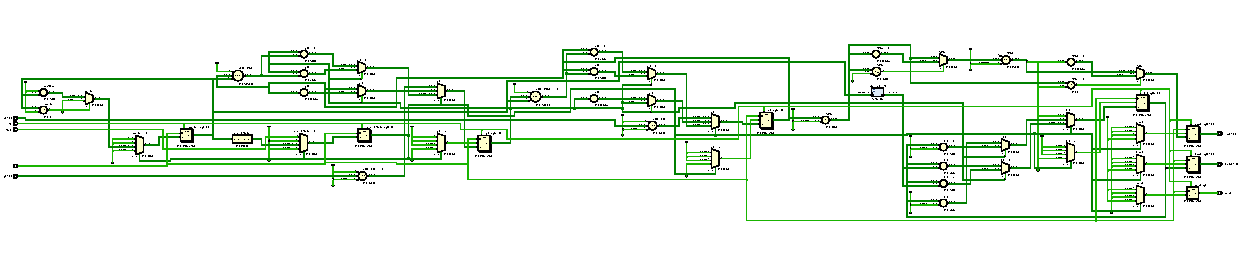
\includegraphics[width=\textwidth]{./images/Synthesis/schematic.pdf}
    \caption{Elaborated RTL design.}
    \label{fig:schematic}
\end{figure}

\section{Synthesis and Implementation}
The Synthesis runs successfully without any errors, 
but a warning is reported regarding I/O constraints. 
The Timing Constraints are verified against a 20 ns clock period (50 MHz frequency), 
meeting the desired specifications. The 
Implementation also completes successfully; however, a 
warning (UCIO \#1) is raised, indicating that all 68 
logical ports lack user-assigned specific location 
constraints (LOC). This warning highlights potential 
risks such as I/O contention, board power or connectivity 
issues, performance degradation, signal integrity problems, 
or, in extreme cases, damage to the device or connected 
components. However, the assignment of specific pin 
locations was outside the scope of this project and was 
therefore not addressed.




